\documentclass[a4paper,12pt]{article} % тип документа
\usepackage{wrapfig}
\usepackage{tikz}
\usepackage[T2A]{fontenc}			% кодировка
\usepackage[utf8]{inputenc}			% кодировка исходного текста
\usepackage[english,russian]{babel}	% локализация и переносы
\usepackage{amsfonts,longtable}
% Математика
\usepackage{amsmath,amsfonts,amssymb,amsthm,mathtools} 


\usepackage{wasysym}
\title{Вопрос по выбору по курсу \\ <<Общая физика>>  \\ 
\vspace{0.2cm}
\vspace{4.5cm}
 \LARGE{\textbf{<<Маятник Капицы>>}}\vspace{5.5cm}}
\date{29.12.2018}
\usepackage{tikz}
\author{\vspace{0.2cm}Баринов Леонид 827 группа}

\begin{document}
\maketitle
\newpage
\section{Изучаемая физическая система}
Когда частота вынужденных осцилляций точки подвеса приблизительно вдвое больше частоты собственных колебаний маятника, нижнее положение равновесия становится неустойчивым: амплитуда первоначально сколь угодно малых колебаний маятника начинает прогрессивно нарастать со временем. Это хорошо известное явление называется параметрическим резонансом.

Интересная черта в поведении жесткого маятника с осциллирующим подвесом заключается в динамической стабилизации перевернутого положения равновесия. При достаточно больших значениях частоты и амплитуды осцилляций подвеса приведенный в перевернутое положение маятник не обнаруживает тенденции к опрокидыванию. Более того, при умеренных отклонениях от вертикали маятник стремится к этому перевернутому положению. Если маятник отклонить от вертикали, он будет совершать сравнительно медленные колебания около перевернутого положения на фоне быстрых осцилляций подвеса. На это теперь широко известное предсказание классической механики впервые, по-видимому, обратил внимание А. Стефенсон еще в 1908 году. Физическое объяснение динамической стабилизации перевернутого маятника было предложено академиком Петром Леонидовичем Капицей в 1951 году, выполнившим также и детальное экспериментальное исследование этого явления. Приведем цитату из статьи Капицы, опубликованной в журнале «Успехи физических наук»:

«Демонстрация явления колебания перевернутого маятника весьма эффектна, быстрые мелкие передвижения, вызванные вибрациями, не заметны на-глаз, поэтому поведение маятника в перевернутом положении производит на зрителя неожиданное впечатление . . . Если осторожно прикасаться пальцем к стержню маятника и отводить его в сторону, то палец чувствует давление, производимое вибрационным моментом. После ознакомления на опыте с динамической устойчивостью маятника в перевернутом положении трудно не прийти к выводу, что она так же поучительна, как и динамическая устойчивость волчка, и ей также следует занять почетное место в лектории на демонстрациях по механике.»

Для демонстрации этого явления можно использовать старую электробритву вибрационного типа, как показано на рис. 1. К вибратору прикреплен удлинитель для увеличения амплитуды осцилляций подвеса маятника. Легкий жесткий стержень маятника соединен с концом удлинителя через шарнир. Корпус бритвы удерживается рукой в таком положении, чтобы вибрация оси происходила в вертикальном направлении. Если стержень маятника привести в вертикальное перевернутое положение, он остается в этом положении до тех пор пока ось вибрирует. Если стержень маятника немного отвести в сторону и отпустить, наблюдаются колебания около перевернутого положения.


\begin{figure}[h]
\centering
\includegraphics[scale=0.4]{1}
\caption{Демонстрация динамической стабилизации перевернутого маятника.}
\end{figure}
\section{Параметрический резонанс}
Будем для простоты рассматривать маятник в виде легкого жесткого стержня длиной $l$ с грузом (точечной массой) $m$ на конце, считая, что именно здесь сосредоточена вся масса маятника. Сила тяжести $mg$ создает возвращающий момент --$mgl\sin\varphi$, пропорциональный синусу угла отклонения $\varphi$ маятника от положения равновесия. Когда подвес маятника неподвижен, этот момент заставляет отклоненный маятник совершать колебания относительно нижнего положения устойчивого равновесия. Если же подвес принудительно движется с некоторым ускорением, поведение маятника удобно описывать с помощью неинерциальной системы отсчета, связанной с подвесом. Из-за ускоренного движения такой системы отсчета на все тела, наряду с «обычными» силами, действует еще и сила инерции, направленная противоположно ускорению системы отсчета. Допустим, что подвес осциллирует вдоль вертикали и его координата $z(t)$ изменяется со временем по гармоническому закону с некоторой частотой $\omega$ и амплитудой $a$:
\begin{equation}
z(t) = a\cos\omega t \qquad
\text{или} \qquad
z(t) = a\sin\omega t 
\end{equation}

В зависимости от характера решаемой задачи в (1) может оказаться удобным тот или иной выбор начальной фазы осцилляций подвеса (выбор начала отсчета времени). Приложенная к грузу маятника сила инерции $F_{in}(t)$ также зависит от времени по синусоидальному закону:
\begin{equation}
F_{in}(t) = -m\frac{d^2z(t)}{dt^2} = -m\ddot{z}(t) = m\omega^2 z(t)
\end{equation}

Сила инерции направлена вниз в течение тех интервалов времени, когда осциллирующий подвес находится ниже своего среднего положения, т.е. когда $z(t) < 0$. Это непосредственно видно из выражения (2) для $F_{in}(t)$, правая часть которого зависит от времени так же, как и $z$-координата подвеса. Поэтому на протяжении соответствующей половины периода колебаний подвеса действие силы инерции равносильно некоторому увеличению силы тяжести. На протяжении другой половины периода, когда подвес находится выше среднего положения (когда $z(t) > 0$), сила инерции направлена вверх, что равносильно уменьшению силы тяжести.

Принимая во внимание такое периодическое изменение (модуляцию) эффективной силы тяжести, легко понять причину раскачки маятника при параметрическом резонансе, когда два цикла модуляции происходят на протяжении одного периода собственных колебаний (рис. 2). В самом деле, пусть при движении маятника к положению равновесия от точки наибольшего отклонения (это четверть собственного периода) осциллирующий подвес все время находится ниже среднего положения, т.е. $z(t) < 0$ (что занимает половину периода осцилляций). Благодаря увеличению эффективной силы тяжести маятник придет к положению равновесия с большей скоростью, чем в отсутствие осцилляций подвеса. В момент прохождения маятником вертикального положения движущийся вверх подвес пересекает свое среднее положение. При движении маятника к точке наибольшего отклонения осциллирующий подвес находится выше среднего положения ($z(t) > 0$, рис. 2), что, как мы видели, равносильно уменьшению силы тяжести. В результате маятник отклонится на больший угол, чем при неподвижном подвесе. При обратном движении к положению равновесия эффективная сила тяжести опять увеличивается, и маятник набирает еще большую скорость, и т.д. Для наиболее интенсивной раскачки частота принудительных осцилляций подвеса должна быть вдвое больше частоты собственных колебаний маятника, и фазовые соотношения должны быть такими, чтобы в моменты прохождения маятником положения равновесия подвес двигался вверх и пересекал свое среднее положение.

Увеличение энергии маятника происходит за счет работы, совершаемой источником, возбуждающим осцилляции подвеса. Размах колебаний растет, если вложение энергии за период превосходит потери из-за трения, т.е. когда амплитуда принудительных осцилляций подвеса превосходит некоторое пороговое значение. В отличие от обычного резонанса, возбуждаемого прямым воздействием периодической силы и происходящего при совпадении ее частоты с собственной частотой маятника, при параметрическом резонансе трение не в состоянии ограничить рост амплитуды. Размах установившихся колебаний маятника оказывается конечным из-за того, что с ростом амплитуды в этой нелинейной системе возрастает период собственных колебаний. При неизменном периоде осцилляций точки подвеса возрастание собственного периода приводит к нарушению условий параметрического резонанса. Амплитуда начинает убывать, условия резонанса снова восстанавливаются, что опять приводит к росту амплитуды, и так далее. Из-за трения такие переходные биения постепенно затухают, и в конце концов устанавливаются периодические колебания неизменного размаха.
\begin{figure}[h]
\centering
\includegraphics[scale=0.35]{5}
\caption{График угла отклонения, фазовая траектория (c сечениями Пуанкаре) и траектория груза маятника в пространстве при параметрическом резонансе. Шкала времени проградуирована в периодах принудительных осцилляций подвеса.}
\end{figure}

В нижней части рис. 2 слева приведена фазовая траектория резонансной раскачки маятника. Сечения Пуанкаре на ней показывают состояние маятника в моменты времени, когда осциллирующий подвес находится в крайнем нижнем положении. В процессе установления колебаний раскручивающаяся фазовая траектория приближается к замкнутой кривой — предельному циклу, соответствующему периодическому процессу, а множество сечений Пуанкаре стягивается к двум неподвижным точкам на фазовой плоскости. Внизу справа на рис. 2 показана траектория груза маятника в пространстве для процесса параметрической раскачки.

Показанные на рис. 2 график и фазовая траектория получены численным интегрированием дифференциального уравнения для угла отклонения $\varphi(t)$ маятника с осциллирующим подвесом. В это уравнение, наряду с моментом силы тяжести $mg$ ($g$ — ускорение свободного падения), включен момент силы инерции $F_{in}(t)$, который явно зависит от времени $t$:
\begin{equation}
\ddot{\varphi} + 2\gamma\dot{\varphi} + \left(\frac{g}{l} - \frac{a}{l}\omega^2\cos\omega t\right)\sin\varphi = 0
\end{equation}

Второй член в (3) учитывает момент силы трения, который в этой модели принят пропорциональным мгновенному значению угловой скорости маятника $\dot\varphi$. Постоянная затухания $\gamma$ обратно пропорциональна добротности $Q$, которую обычно используют для характеристики затухания малых собственных колебаний под действием вязкого трения: $Q = \omega_0/2\gamma$, где  $\omega_0 = g/l$  — частота собственных колебаний предельно малой амплитуды в отсутствие осцилляций подвеса.

Отметим, что колебания около перевернутого положения можно формально описывать тем же самым дифференциальным уравнением (3) с отрицательными значениями $g$. Иными словами, в уравнении (3) ускорение свободного падения $g$ можно рассматривать как управляющий параметр, изменение которого физически эквивалентно изменению действующей на маятник силы тяжести. Когда этот параметр уменьшается до нуля и дальше в область отрицательных значений, не зависящий от времени (обусловленный силой тяжести) момент в уравнении (3) сначала обращается в нуль, а затем изменяет знак на противоположный. Подобная обращенная по направлению «сила тяжести» стремится привести маятник в перевернутое положение $\varphi = \pi$, отчего (в отсутствие вибраций подвеса) оно становится устойчивым, а положение $\varphi = 0$ — неустойчивым: при $g < 0$ верхнее положение маятника в уравнении (3) эквивалентно нижнему положению при положительном значении $g$.
\newpage
\section{Динамическая стабилизация перевернутого маятника}
Для физического объяснения эффекта динамической стабилизации перевернутого маятника при быстрых осцилляциях подвеса нужно принять во внимание действие на маятник силы инерции, усредненное по периоду этих быстрых осцилляций. Согласно формуле (2) сила инерции изменяется со временем по синусоидальному закону, её среднее за период значение равно нулю. Но оказывается, что среднее значение момента этой силы относительно оси вращения маятника отлично от нуля. Именно средний момент силы инерции отвечает за необычное, противоречащее нашей интуиции поведение маятника
\begin{figure}[h]
\centering
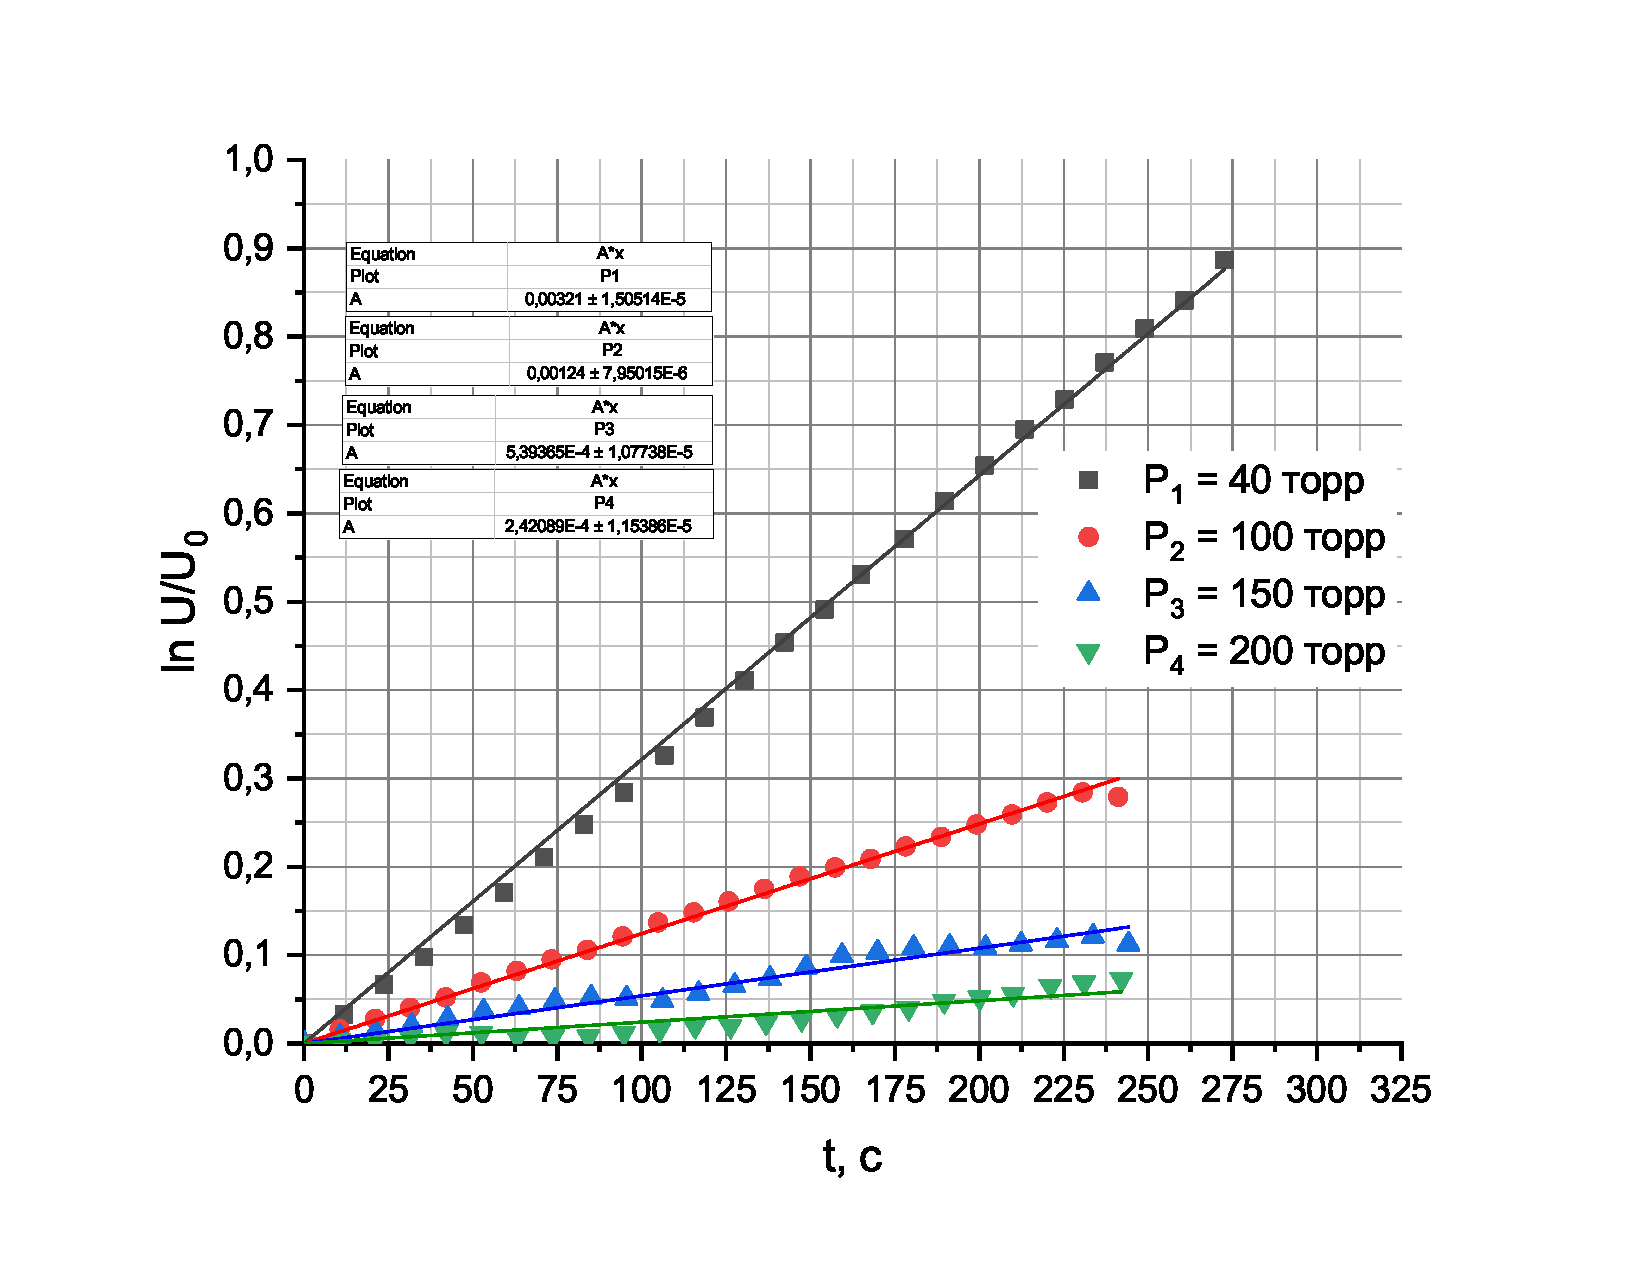
\includegraphics[scale=0.4]{6}
\caption{Силы инерции $F_1$ и $F_2$, действующие на маятник в неинерциальной системе отсчета, в моменты времени, когда осциллирующая ось A находится в крайних положениях 1 и 2 соответственно.}
\end{figure}

Чтобы было проще понять влияние силы инерции на маятник, забудем на некоторое время о силе тяжести. Начнем наш анализ со случая, когда стержень маятника отклонен в горизонтальное положение, т.е. ориентирован под прямым углом $\psi = \pi/2$ к направлению осцилляций подвеса (см. рис. 3,а). Если начальная скорость груза равна нулю, то в инерциальной системе отсчета в отсутствие силы тяжести он будет оставаться на том же уровне, в то время как ось A осциллирует между крайними точками 1 и 2. При этом стержень маятника поворачивается вниз и вверх на небольшой угол, как показано в верхней части рис. 3,а. В неинерциальной системе отсчета, связанной с осью маятника, это же движение стержня маятника показано в нижней части рис. 3,а: груз маятника движется вверх-вниз по дуге и оказывается в крайних точках, когда ось занимает положения 1 и 2. В положении 1 приложенная к грузу сила инерции $F_1$ направлена вверх, а в другом крайнем положении 2 такая же по величине сила $F_2$ направлена вниз. Плечо силы инерции в положениях 1 и 2 одинаково, поэтому момент этой силы, усредненный за период осцилляций оси, равен нулю. Это значит, что в отсутствие силы тяжести такая ориентация стержня маятника (перпендикулярно к направлению осцилляций оси) соответствует положению динамического равновесия (неустойчивому, как будет показано ниже).

Теперь рассмотрим случай, когда стержень маятника в среднем отклонен на произвольный угол $\psi$ от направления осцилляций подвеса. Пусть ось A перемещается между крайними точками 1 и 2, как показано в верхней части рис. 3,б. В неинерциальной системе отсчета, связанной с подвесом, груз маятника движется вверх-вниз по дуге, центр которой совпадает с осью A. Груз оказывается в крайних точках, когда ось занимает положения 1 и 2, как показано в нижней части рис. 3,б.

Отметим, что мгновенная ориентация стержня маятника в момент 1 одинакова в обеих системах отсчета. В момент 2 (как и в любой другой момент) ориентация стержня также одинакова. Когда ось смещена вверх (в точку 1) из своего среднего положения, действующая на груз маятника сила инерции $F_1$ также направлена вверх. В другом крайнем положении 2 сила инерции $F_2$ направлена вниз. Силы инерции $F_1$ и $F_2$ в крайних положениях оси одинаковы по величине, но момент силы инерции $F_1 $ в положении 1 больше, чем момент силы инерции $F_2$ в положении 2, поскольку плечо силы $F_1$ больше, чем силы $F_2$. Это легко видеть из рис. 3,б. Поэтому в среднем за период осцилляций оси сила инерции создает момент, который стремится повернуть маятник вверх, в вертикальное перевернутое положение, в котором стержень маятника ориентирован вдоль направления осцилляций оси. Если бы стержень маятника был отклонен на некоторый (острый) угол от нижнего вертикального положения, то средний момент силы инерции стремился бы повернуть стержень маятника вниз.

Таким образом, момент силы инерции, усредненный по периоду быстрых осцилляций оси, стремится установить стержень маятника по направлению принудительных колебаний подвеса. П.Л. Капица назвал этот ориентирующий момент вибрационным, но в равной мере справедливо называть этот момент инерционным, потому что его происхождение обусловлено силой инерции, возникающей в связанной с подвесом системе отсчета из-за быстрых осцилляций оси маятника. Именно средний момент силы инерции дает наглядное объяснение существованию двух устойчивых положений равновесия маятника, соответствующих его ориентации вдоль направления колебаний оси. При заданных значениях частоты и амплитуды колебаний подвеса этот средний момент, как и момент силы тяжести, зависит только от угла отклонения маятника. В поле тяжести перевернутый маятник устойчив по отношению к малым отклонениям от вертикали при условии, что средний момент силы инерции больше, чем опрокидывающий момент силы тяжести.
\section{Приближенная количественная теория перевернутого маятника}
На основе приведенной выше наглядной картины можно сформулировать количественный критерий динамической стабилизации перевернутого маятника. При быстрых осцилляциях точки подвеса движение маятника можно представить, следуя П.Л. Капице, как суперпозицию двух компонент: медленного движения, для которого характерно малое изменение угла ориентации стержня за период вынужденных осцилляций оси, и быстрого («вибрационного») движения.

Когда стержень маятника отклонен от нижнего положения равновесия в среднем на угол $\psi$, мгновенное значение угла отклонения $\varphi(t)$ из-за принудительных осцилляций оси подвержено быстрым синусоидальным колебаниям с частотой $\omega$ около этого среднего значения $\psi = \langle\varphi(t)\rangle$. Это ясно видно из графиков зависимости угла отклонения $\varphi(t)$ от времени, показанных ниже на рис. 4. Поэтому можно искать мгновенное значение угла отклонения $\varphi(t)$ как сумму медленно изменяющейся функции $\psi(t)$ и быстрого слагаемого $\delta(t)$, среднее значение которого равно нулю. Быстрый член $\delta(t)$ совершает колебания с высокой частотой $\omega$ принудительных колебаний оси. Как видно из рис. 3,б, угловая амплитуда этих быстрых колебаний пропорциональна синусу среднего угла отклонения $\psi$:
\begin{equation}
\varphi(t) = \psi(t) + \delta(t) = \psi(t) - \frac{z(t)}{l}\sin\psi = \psi(t) - \frac{a}{l}\sin\psi\cos\omega t
\end{equation}
Здесь использовано выражение (1) для мгновенного положения оси $z(t)$, в котором $a$ — амплитуда принудительных колебаний оси, $l$ — длина маятника. Знак второго слагаемого в (4) объясняется тем, что когда ось находится выше своего среднего положения, т.е. значение $z$ положительно, дополнительный угол $\delta$ = $-(z/l)\sin\psi$ отрицателен, и наоборот. Ниже мы получим дифференциальное уравнение для искомой медленно изменяющейся функции $\psi(t)$, которая описывает движение маятника, усредненное по периоду быстрых осцилляций.

Момент силы инерции зависит от ее мгновенного значения $ma\omega^2 \cos\omega t$ (см. (2)) и от синуса угла $\varphi$. Осцилляции оси приводят лишь к небольшим отклонениям угла $\varphi$ от его среднего значения $\psi$ (т.е. $\delta(t) \ll 1$ для любого $t$), поэтому для синуса угла $\varphi$ можно написать следующее приближенное выражение:
\begin{equation}
\sin\varphi = \sin(\psi + \delta) \approx \sin\psi + \delta\cos\psi
\end{equation}
\begin{figure}[h]
\centering
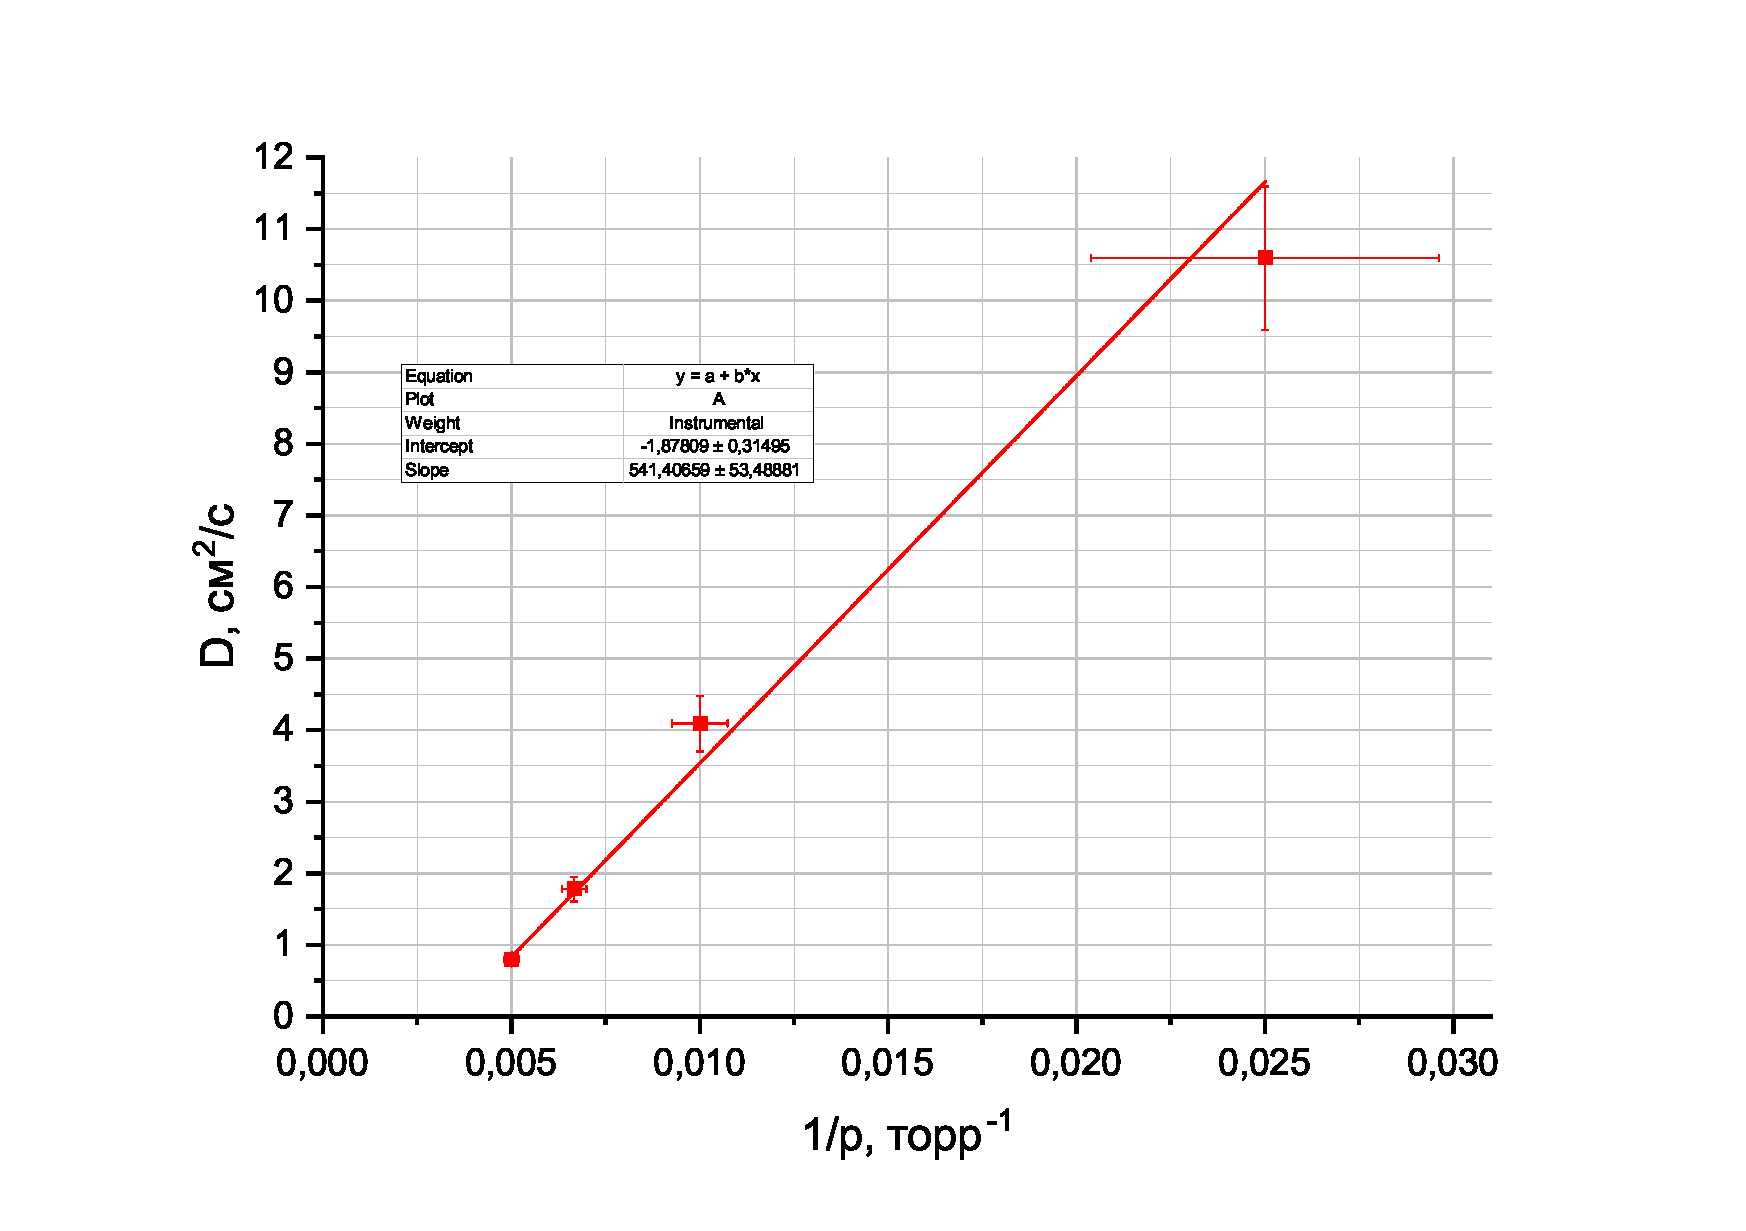
\includegraphics[scale=0.35]{7}
\caption{Графики угла отклонения $\varphi(t)$ при колебаниях маятника около нижнего и верхнего положений равновесия вместе с графиком $z(t) = -a\cos\omega t$ вынужденных осцилляций оси. Графики получены численным интегрированием дифференциального уравнения (3).}
\end{figure}

Используя это выражение и считая $\psi$ практически неизменным на протяжении периода осцилляций оси, находим приближенное значение момента силы тяжести относительно оси маятника, усредненное по периоду быстрых осцилляций оси:
\begin{equation}
\langle-mgl\sin\varphi\rangle = -mgl\langle\sin(\psi+\delta)\rangle = -mgl\sin\psi
\end{equation}

Здесь учтено, что среднее значение $\delta(t)$ равно нулю: $\langle\delta(t)\rangle = 0$. Таким образом, среднее значение момента силы тяжести будет таким же, как в случае неподвижного подвеса: второй (осциллирующий) член в выражении (4) для мгновенного значения угла отклонения, будучи умноженным на постоянную (не зависящую от времени) силу тяжести, не дает вклада в средний момент сил. Напротив, при усреднении по времени момента осциллирующей силы инерции вклад первого члена разложения (4) обращается в нуль, но второй член дает ненулевой вклад в средний момент. Так происходит благодаря одинаковой синусоидальной зависимости от времени как $\delta(t)$, так и силы инерции $F_{in}(t)$ (см. (2)):
\begin{eqnarray}
\langle F_{in}(t)l\sin(\psi + \delta)\rangle = -ma\omega^2l(a/l)\cos\psi\sin\psi\langle\cos^2\omega t\rangle = \nonumber\\
-\frac{1}{2}ma^2\omega^2\cos\psi\sin\psi = -\frac{1}{4}ma^2\omega^2\sin2\psi
\end{eqnarray}
В (7) учтено, что среднее за период значение квадрата косинуса равно 1/2. В случае $\psi > \pi/2$ средний момент силы инерции положителен: когда маятник образует острый угол с направлением вверх, этот момент стремится повернуть стержень маятника в перевернутое положение. Сравнивая правые части выражений (6) и (7), можно найти условие, при котором момент силы инерции, действующий на отклоненный из перевернутого положения маятник, превосходит момент силы тяжести, стремящейся привести маятник в нижнее положение:
\begin{equation}
a^2\omega^2 > 2gl
\end{equation}
Таким образом, перевернутое положение маятника устойчиво, если максимальная скорость $\omega a$ осциллирующей оси больше, чем скорость $\sqrt{2gl}$, которую тело, свободно падающее в поле тяжести, приобретает при падении с высоты, равной длине маятника $l$. Критерий устойчивости перевернутого маятника (8) можно представить в другой форме, если воспользоваться выражением $\omega_0 = g/l$ для частоты малых собственных колебаний маятника (в отсутствие осцилляций подвеса). Подставляя $g = l\omega_0^2$ в (8), получаем:
\begin{equation}
\frac{a}{l} \cdot\frac{\omega}{\omega_0} > \sqrt{2}
\end{equation}

Согласно критерию (9), произведение безразмерной относительной амплитуды $a/l$ и относительной частоты $\omega/\omega_0$ осцилляций подвеса должно превышать $\sqrt{2}$. Например, для маятника длиной $l = 20$ см при частоте вибраций оси $f = \omega/2\pi = 100$ Гц амплитуда $a$ этих вибраций должна превышать 3.2 мм. Для физического маятника критерий динамической стабилизации перевернутого положения дается такими же выражениями (8) или (9), если в них в качестве $l$ подставлять приведенную длину маятника $I/md$, где $I$ — момент инерции относительно оси вращения, $m$ — масса маятника и $d$ — расстояние от оси вращения до центра масс.

Для заданных значений частоты $\omega$ и амплитуды $a$ осцилляций подвеса, при которых выполнено условие (8) или (9), можно найти максимально допустимое значение среднего отклонения маятника от перевернутого положения $\theta_{max} = \pi — \psi_0$, в пределах которого маятник будет возвращаться в перевернутое положение. Для этого достаточно приравнять правые части выражений (6) и (7), которые определяют средний момент силы тяжести, стремящийся опрокинуть маятник, и средний момент силы инерции, стремящийся вернуть маятник в перевернутое положение:
\begin{equation}
\cos\theta_{max} = -\cos\psi_0 = \frac{2gl}{a^2\omega^2} = 2\left(\frac{\omega_0}{\omega} \frac{l}{a}\right)^2
\end{equation}

Чем больше произведение $\omega а$ частоты и амплитуды осцилляций подвеса, тем ближе к $\pi/2$ максимально допустимое отклонение маятника $\theta_{max}$ от перевернутого положения. Если маятник отклонить на угол, меньший $\theta_{max}$, маятник будет совершать сравнительно медленные колебания около перевернутого положения. Это медленное движение происходит в результате совместного действия среднего момента силы инерции и силы тяжести. На медленное движение маятника налагаются быстрые колебания с частотой вынужденных осцилляций подвеса (рис. 4).
Аналогичное поведение маятника наблюдается и при отклонении от нижнего положения равновесия. Но в этом случае частота медленных колебаний маятника больше, чем около перевернутого положения. Действительно, ведь в этом случае и средний момент силы инерции, и момент силы тяжести стремятся вернуть маятник в нижнее положение. Частота колебаний маятника около нижнего положения увеличивается благодаря осцилляциям подвеса.

\end{document}